\clearpage
\appendix
\phantomsection
\addcontentsline{toc}{section}{Appendix A: Additional Figures}
\section*{Appendix A: Additional Figures}
\setcounter{figure}{0}
\renewcommand{\thefigure}{A\arabic{figure}}
\setcounter{table}{0}
\renewcommand{\thetable}{A\arabic{table}}

\begin{figure}[htbp]
  \centering
  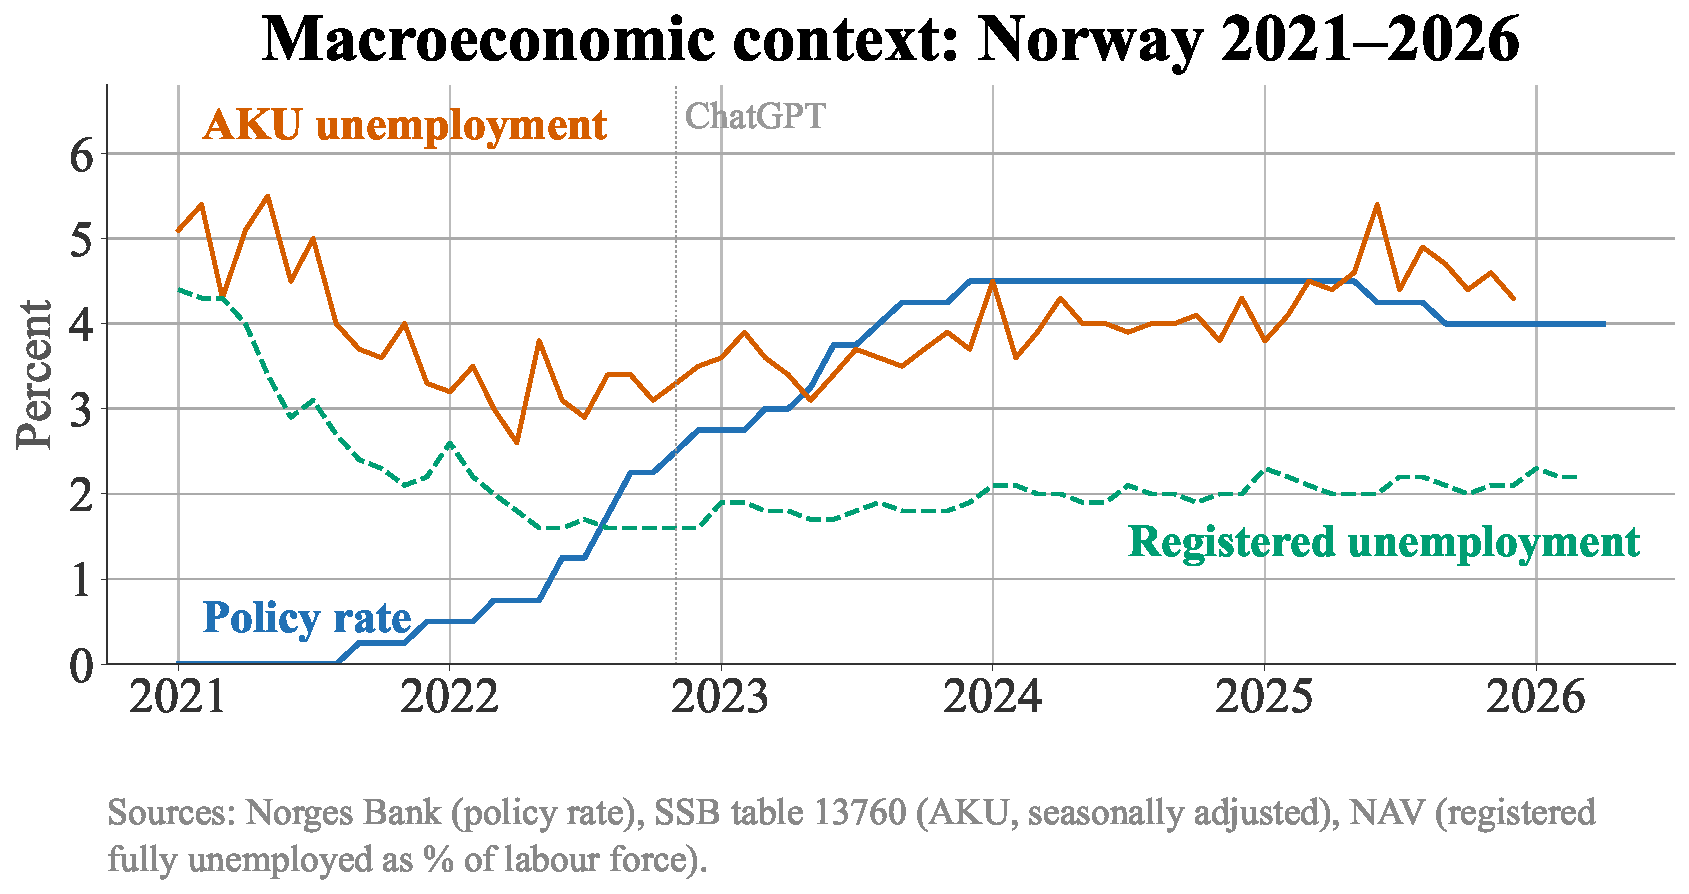
\includegraphics[width=0.8\textwidth]{../analysis/output/figures/figureA0a_macro_context.pdf}
  \caption{Macroeconomic context: Norges Bank policy rate and registered unemployment rate, 2015--2025.}
  \label{fig:macro_context}
\end{figure}

\begin{figure}[htbp]
  \centering
  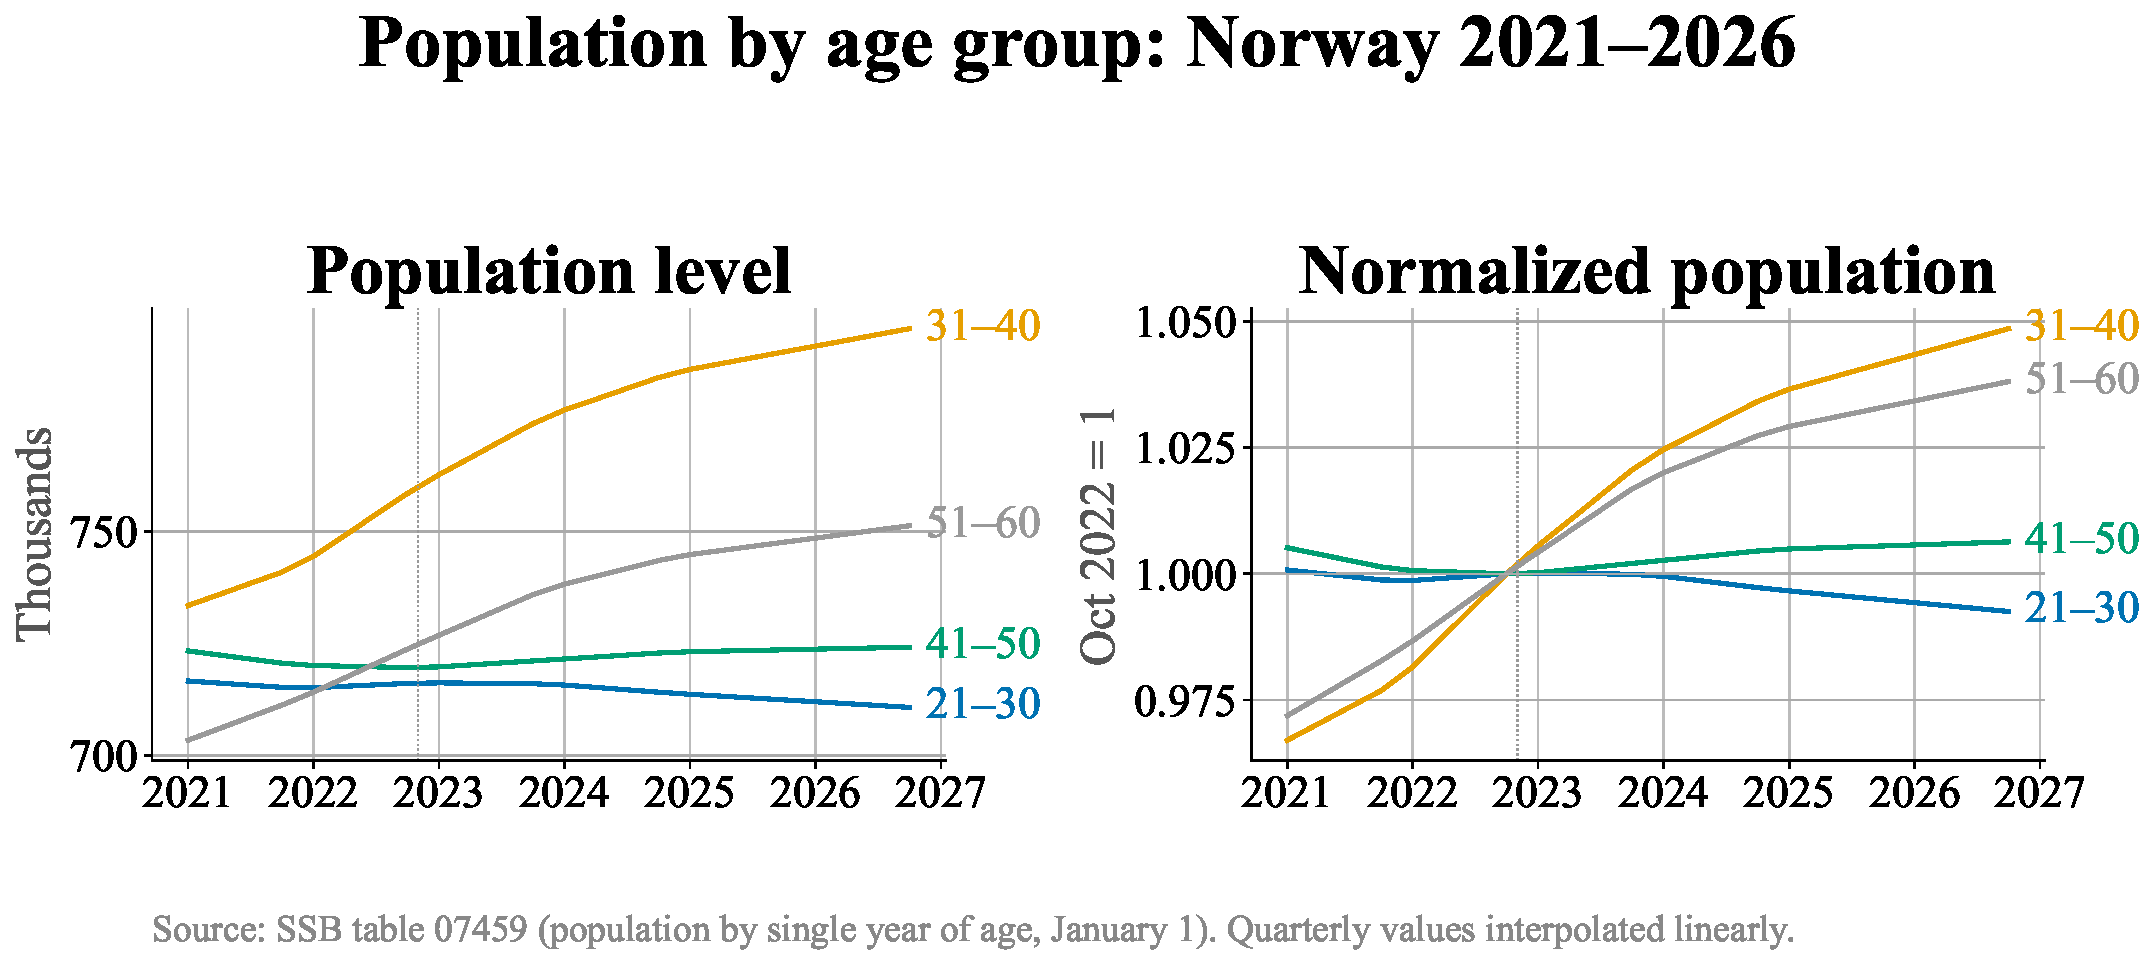
\includegraphics[width=0.8\textwidth]{../analysis/output/figures/figureA0b_cohort_sizes.pdf}
  \caption{Resident population by age group, 2015--2025.}
  \label{fig:cohort_sizes}
\end{figure}

\begin{figure}[htbp]
  \centering
  
\includegraphics[width=\textwidth]{../analysis/output/figures/figure1_occupations_by_age_unadjusted.pdf}
  \caption{Unadjusted employment (raw headcount) in selected occupations by age group, October 2022 = 1. Compare with the population-adjusted Figure~\ref{fig:occupations_by_age} used in the main text.}
  \label{fig:occupations_unadjusted}
\end{figure}

\begin{figure}[htbp]
  \centering
  
\includegraphics[width=\textwidth]{../analysis/output/figures/figure2_age_by_quintile_unadjusted.pdf}
  \caption{Unadjusted employment (raw headcount) by Eloundou et al.\ exposure quintile and age group, October 2022 = 1. Compare with the population-adjusted Figure~\ref{fig:age_by_quintile} used in the main text.}
  \label{fig:quintiles_unadjusted}
\end{figure}

\begin{figure}[htbp]
  \centering
  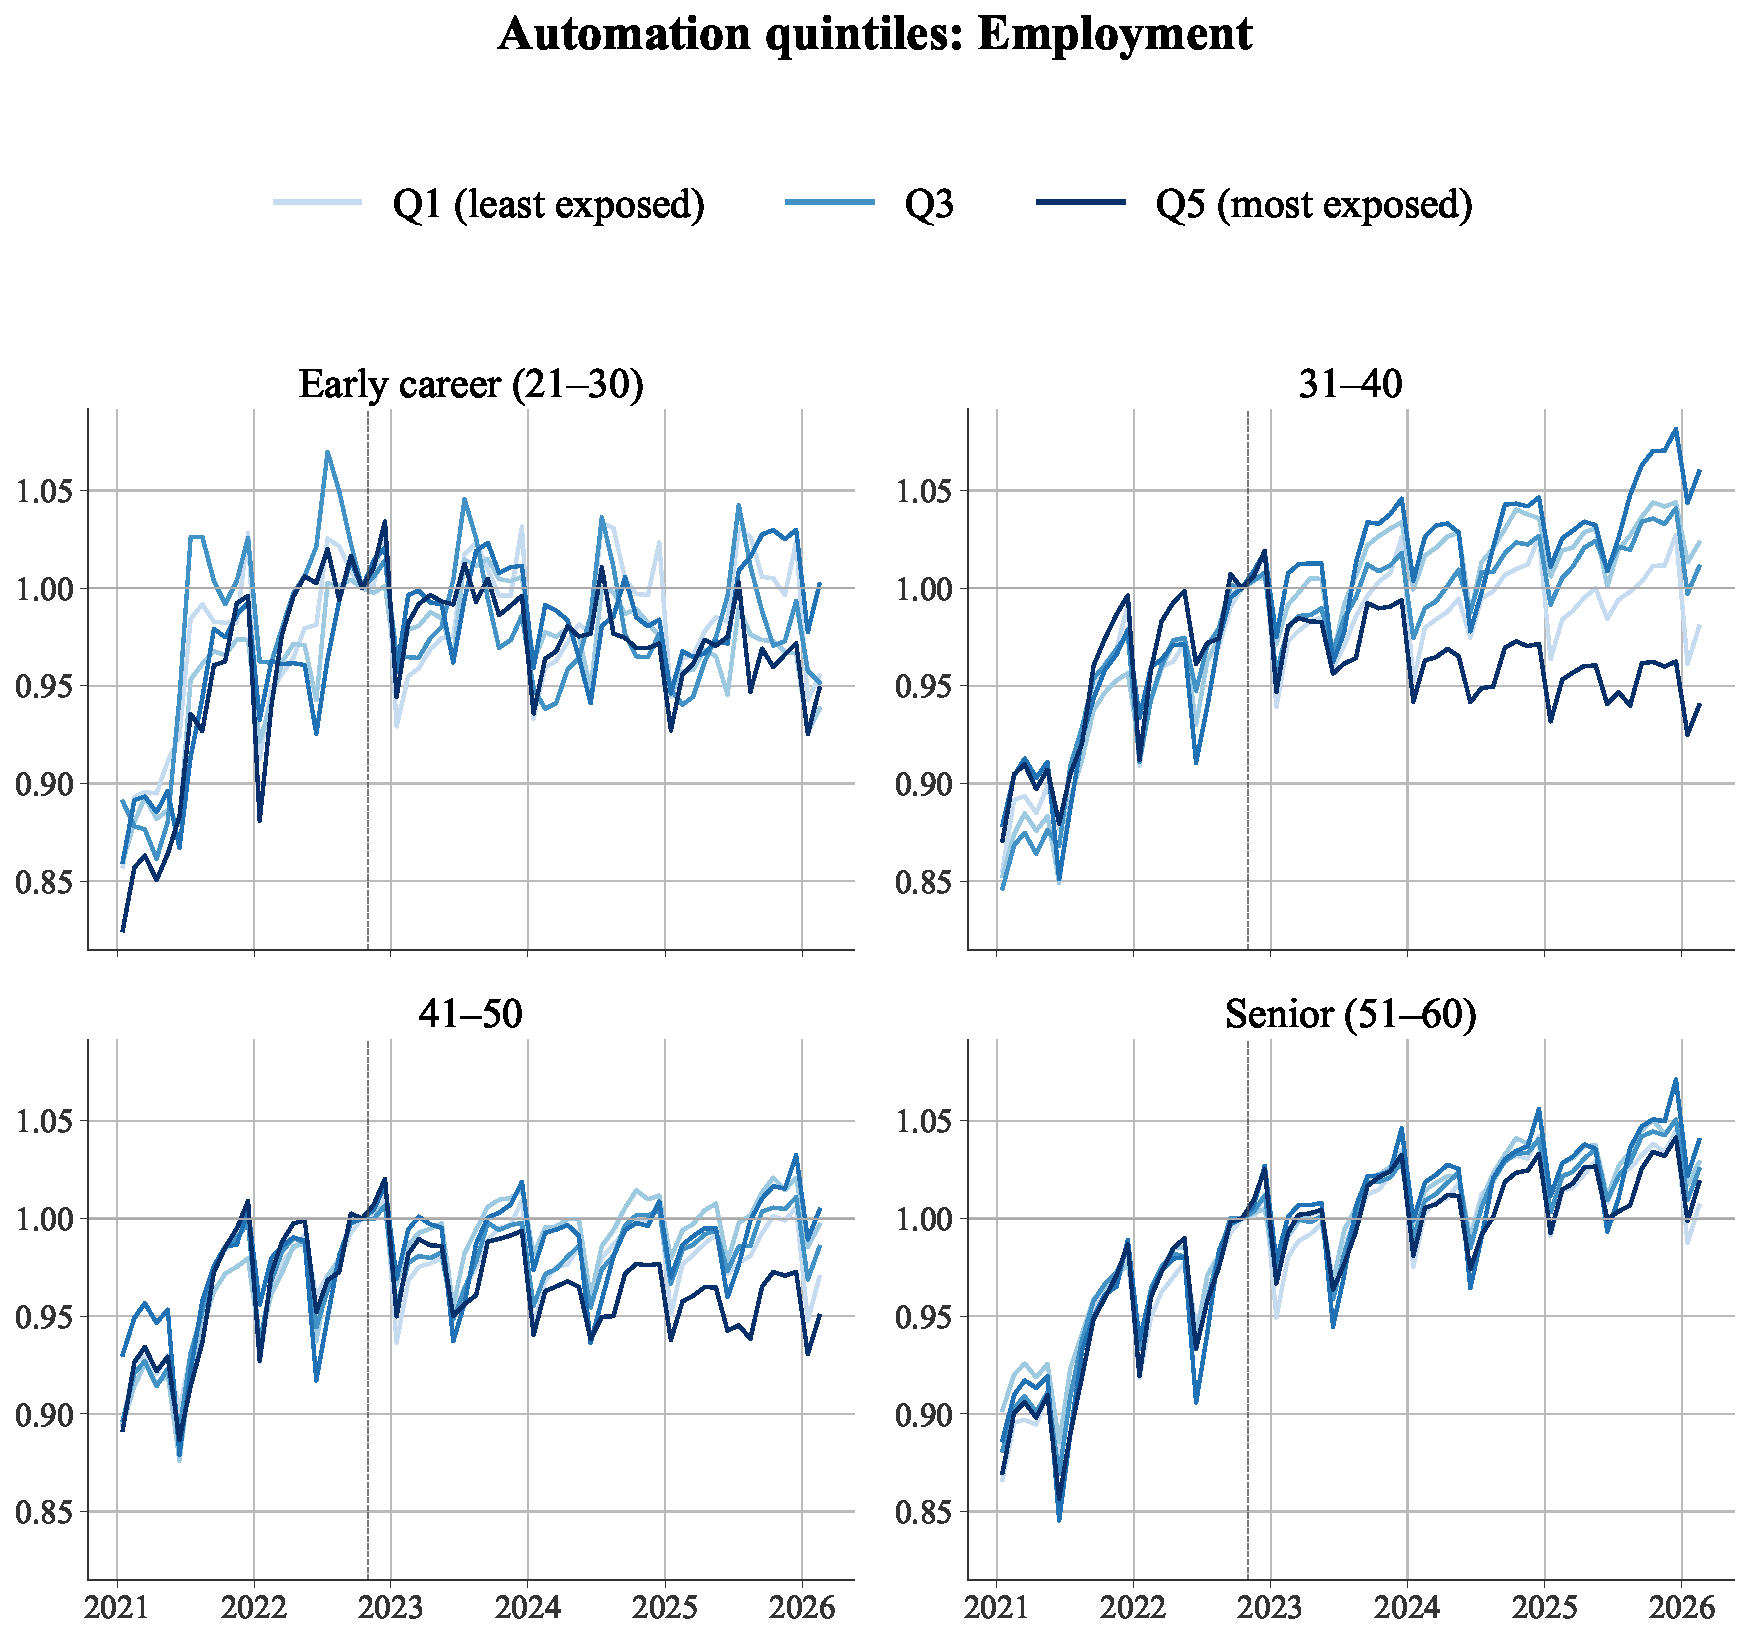
\includegraphics[width=\textwidth]{../analysis/output/figures/figure5b_age_by_quintile_handa.pdf}
  \caption{Employment by age and Handa et al.\ automation exposure quintile, October 2022 = 1.}
  \label{fig:age_by_quintile_handa_auto}
\end{figure}

\begin{figure}[htbp]
  \centering
  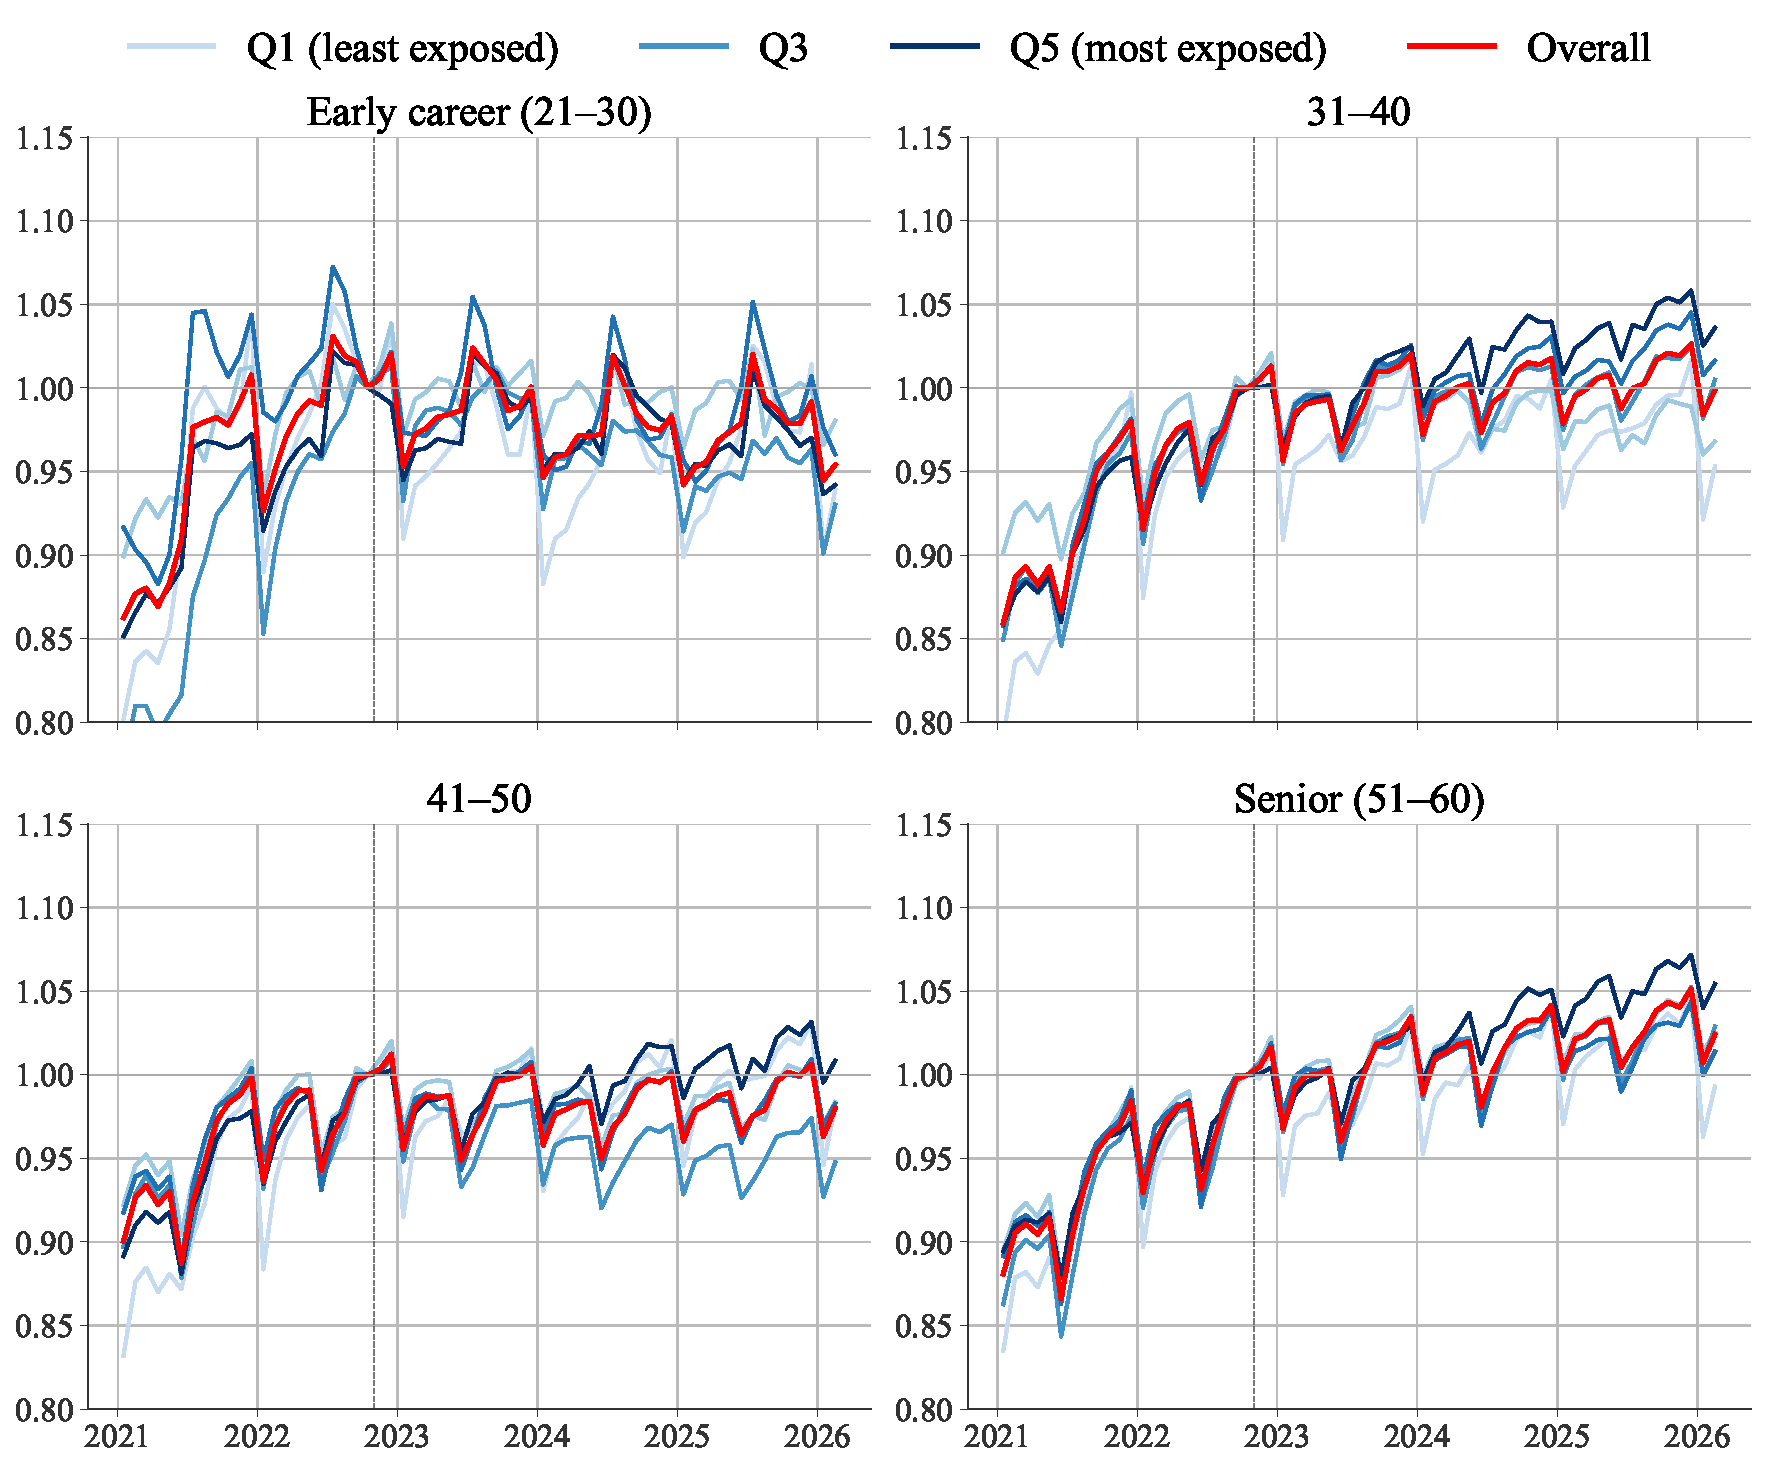
\includegraphics[width=\textwidth]{../analysis/output/figures/figure5c_age_by_quintile_handa.pdf}
  \caption{Employment by age and Handa et al.\ augmentation exposure quintile, October 2022 = 1.}
  \label{fig:age_by_quintile_handa_aug}
\end{figure}

\begin{figure}[htbp]
  \centering
  
\includegraphics[width=\textwidth]{../analysis/output/figures/figure5d_age_by_quintile_job_exposure.pdf}
  \caption{Employment by age and \citet{anthropic2026} \texttt{job\_exposure} quintile, October 2022 = 1. The \texttt{job\_exposure} measure is a time-weighted version of Claude usage with an automation penalty, released by Anthropic in March 2026.}
  \label{fig:age_by_quintile_job_exposure}
\end{figure}

\begin{figure}[htbp]
  \centering
  
\includegraphics[width=\textwidth]{../analysis/output/figures/figure9b_age_by_quintile_felten.pdf}
  \caption{Employment by age and Felten AIOE Language Modeling quintile, October 2022 = 1.}
  \label{fig:age_by_quintile_felten_lm}
\end{figure}

\begin{figure}[htbp]
  \centering
  
\includegraphics[width=\textwidth]{../analysis/output/figures/figureS2_handa_sensitivity.pdf}
  \caption{Crosswalk quality sensitivity for Handa et al.\ overall exposure quintiles.}
  \label{fig:handa_sensitivity}
\end{figure}

\begin{figure}[htbp]
  \centering
  
\includegraphics[width=\textwidth]{../analysis/output/figures/figureS3_handa_auto_sensitivity.pdf}
  \caption{Crosswalk quality sensitivity for Handa et al.\ automation exposure quintiles.}
  \label{fig:handa_auto_sensitivity}
\end{figure}

\begin{figure}[htbp]
  \centering
  
\includegraphics[width=\textwidth]{../analysis/output/figures/figure6a_kontantlonn_by_age.pdf}
  \caption{Monthly earnings by age group for selected occupations. October 2022 = 1.}
  \label{fig:kontantlonn_by_age}
\end{figure}

\begin{figure}[htbp]
  \centering
  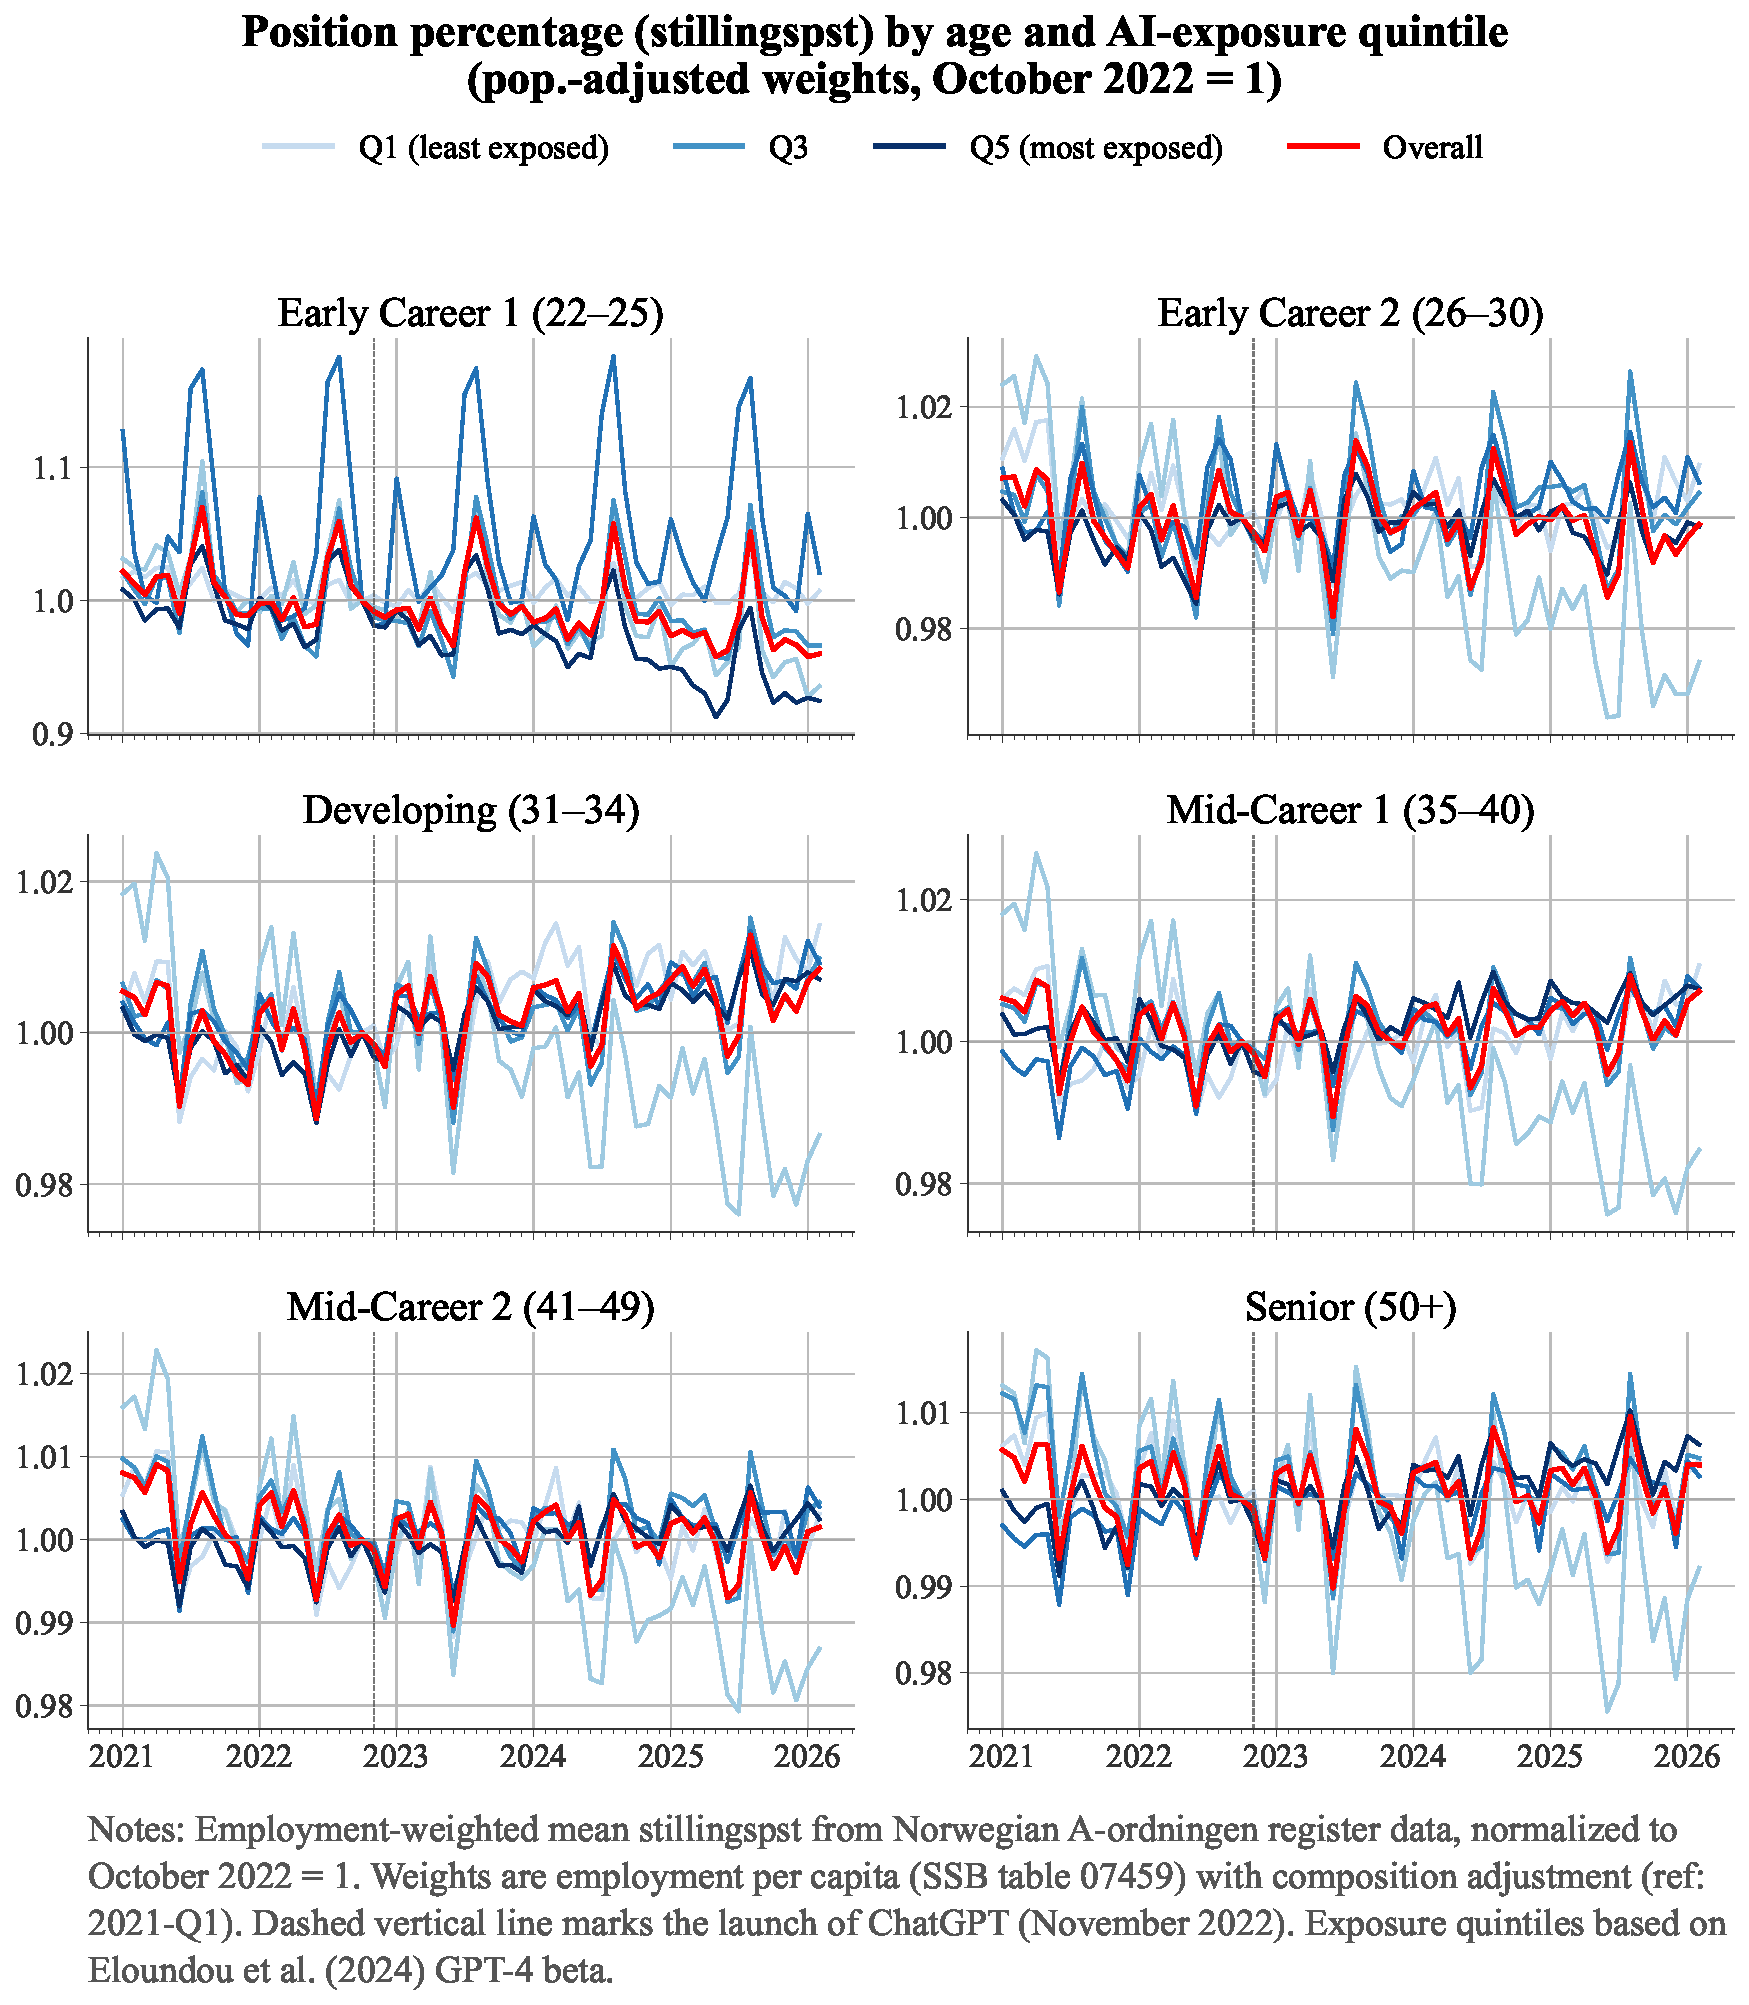
\includegraphics[width=\textwidth]{../analysis/output/figures/figure7b_stillingspst_by_quintile.pdf}
  \caption{Position percentage by Eloundou et al.\ quintile and age group. October 2022 = 1.}
  \label{fig:stillingspst_by_quintile}
\end{figure}

\begin{figure}[htbp]
  \centering
  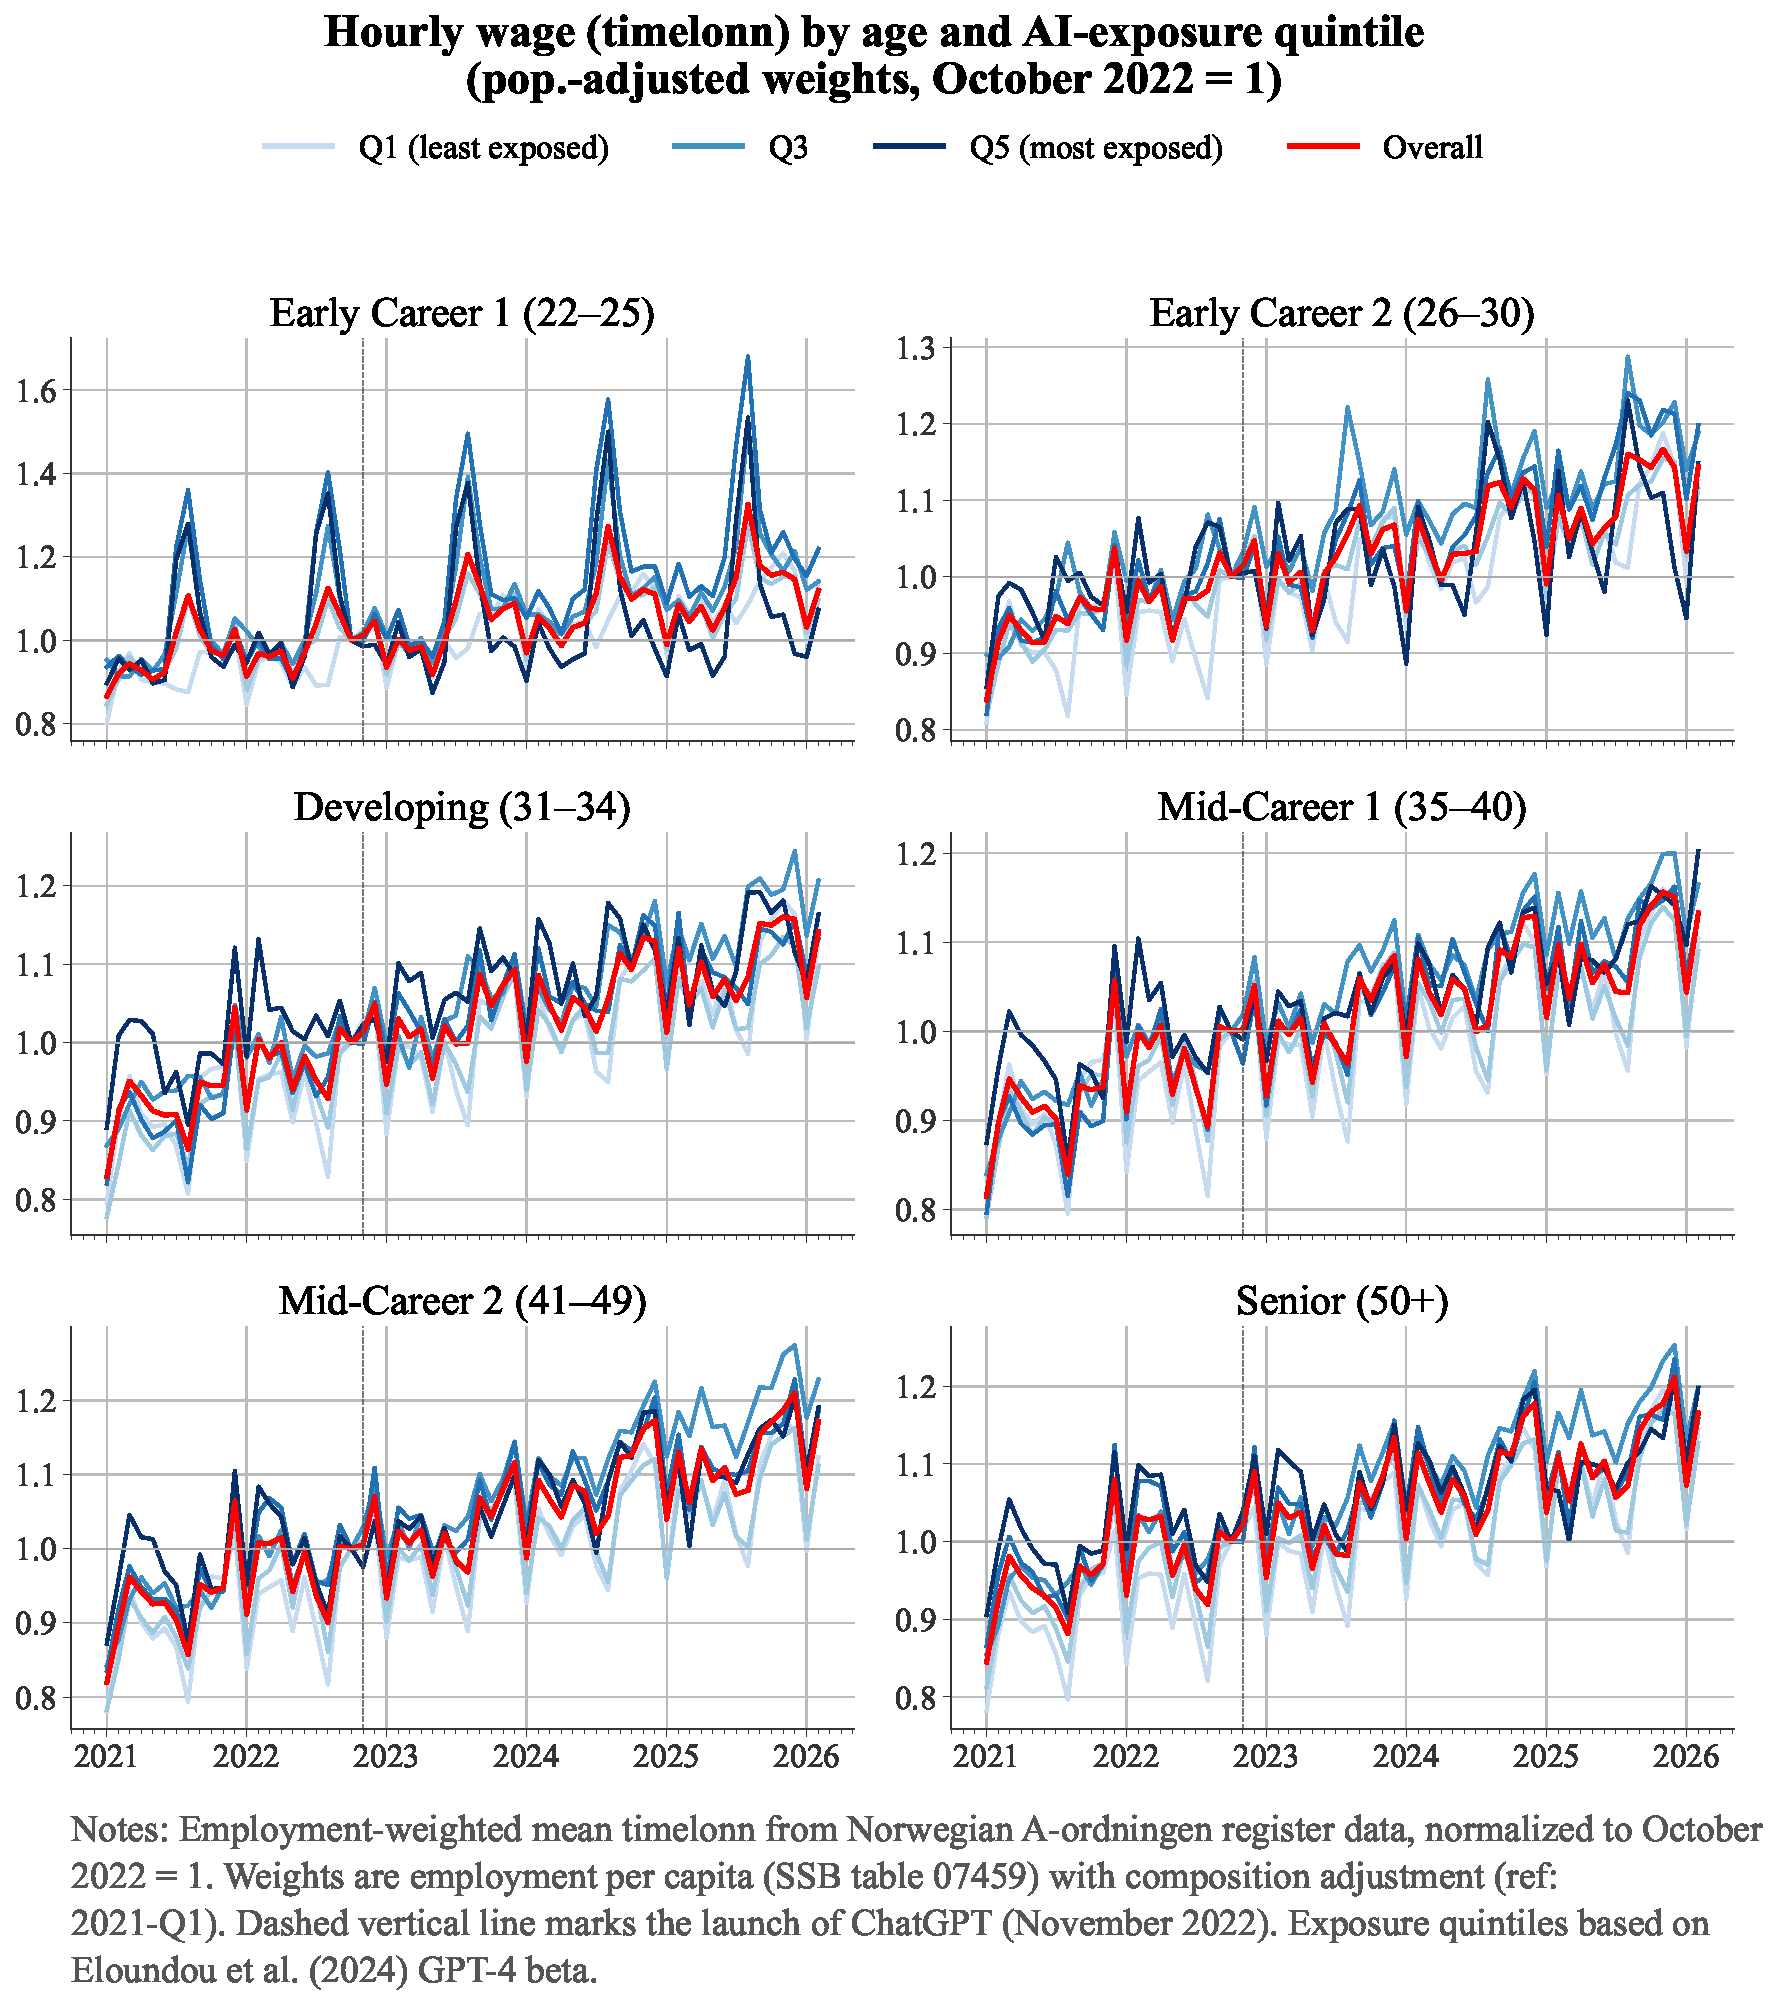
\includegraphics[width=\textwidth]{../analysis/output/figures/figure7c_timelonn_by_quintile.pdf}
  \caption{Hourly wage by Eloundou et al.\ quintile and age group. October 2022 = 1.}
  \label{fig:timelonn_by_quintile}
\end{figure}

\begin{figure}[htbp]
  \centering
  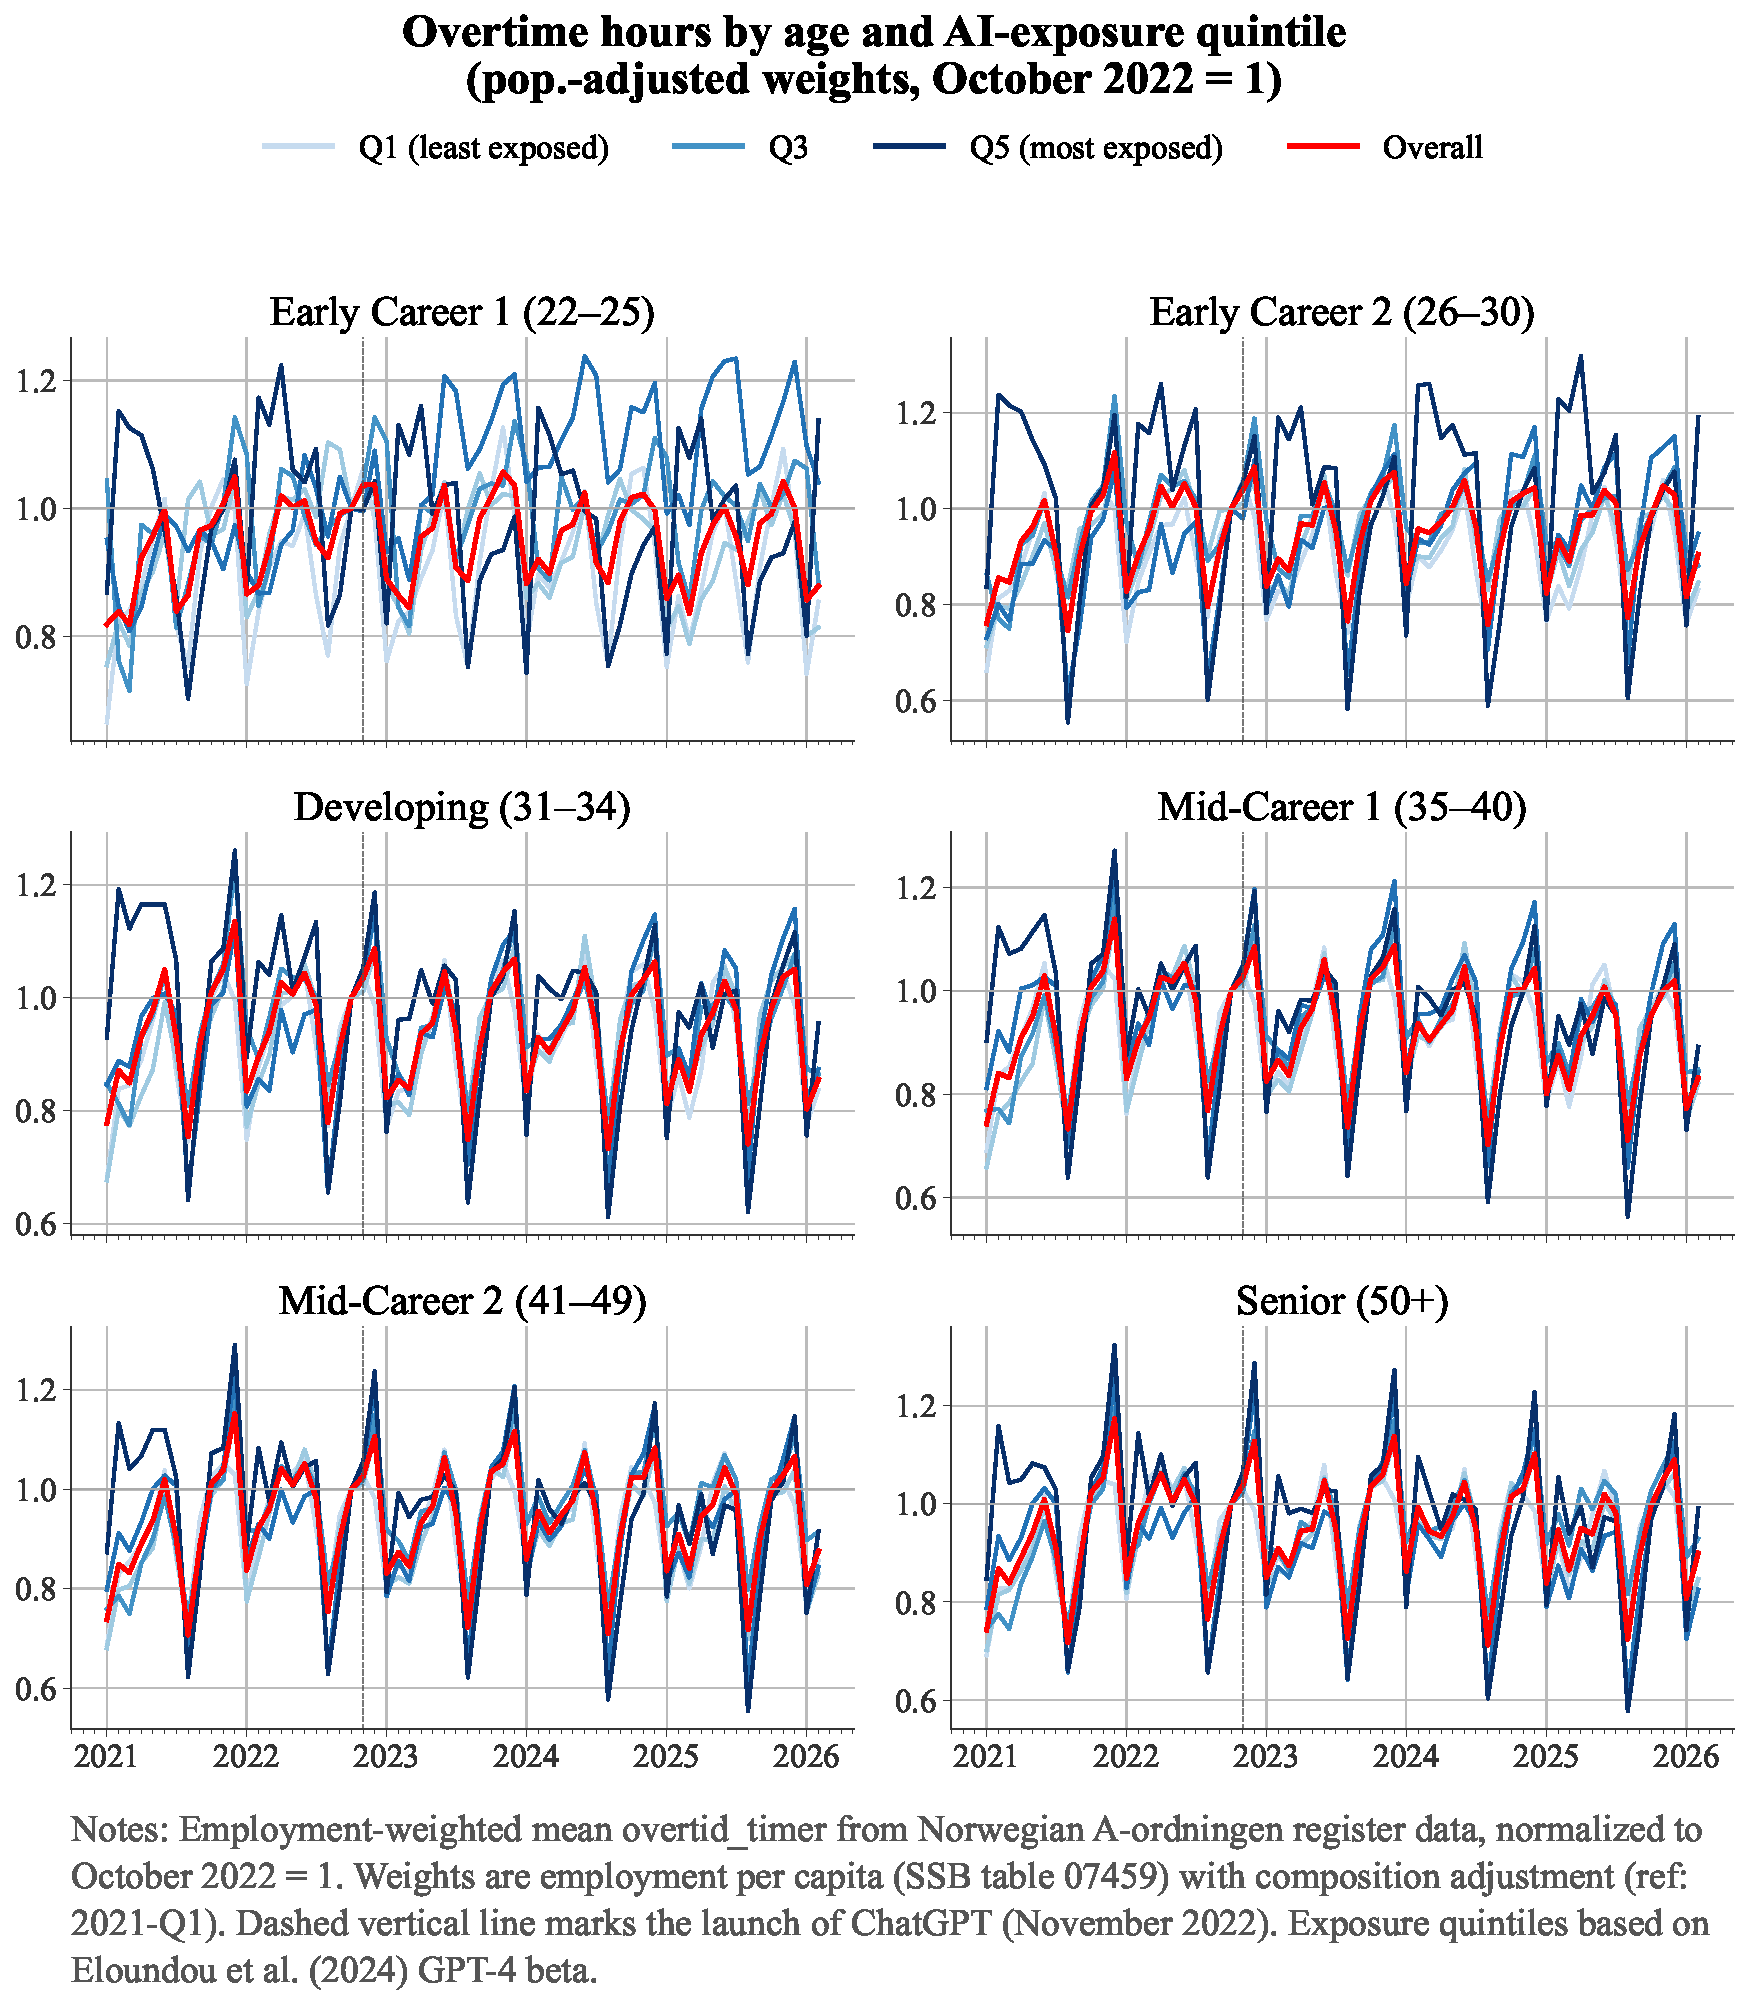
\includegraphics[width=\textwidth]{../analysis/output/figures/figure7d_overtid_timer_by_quintile.pdf}
  \caption{Overtime hours by Eloundou et al.\ quintile and age group. October 2022 = 1.}
  \label{fig:overtid_by_quintile}
\end{figure}

\begin{figure}[htbp]
  \centering
  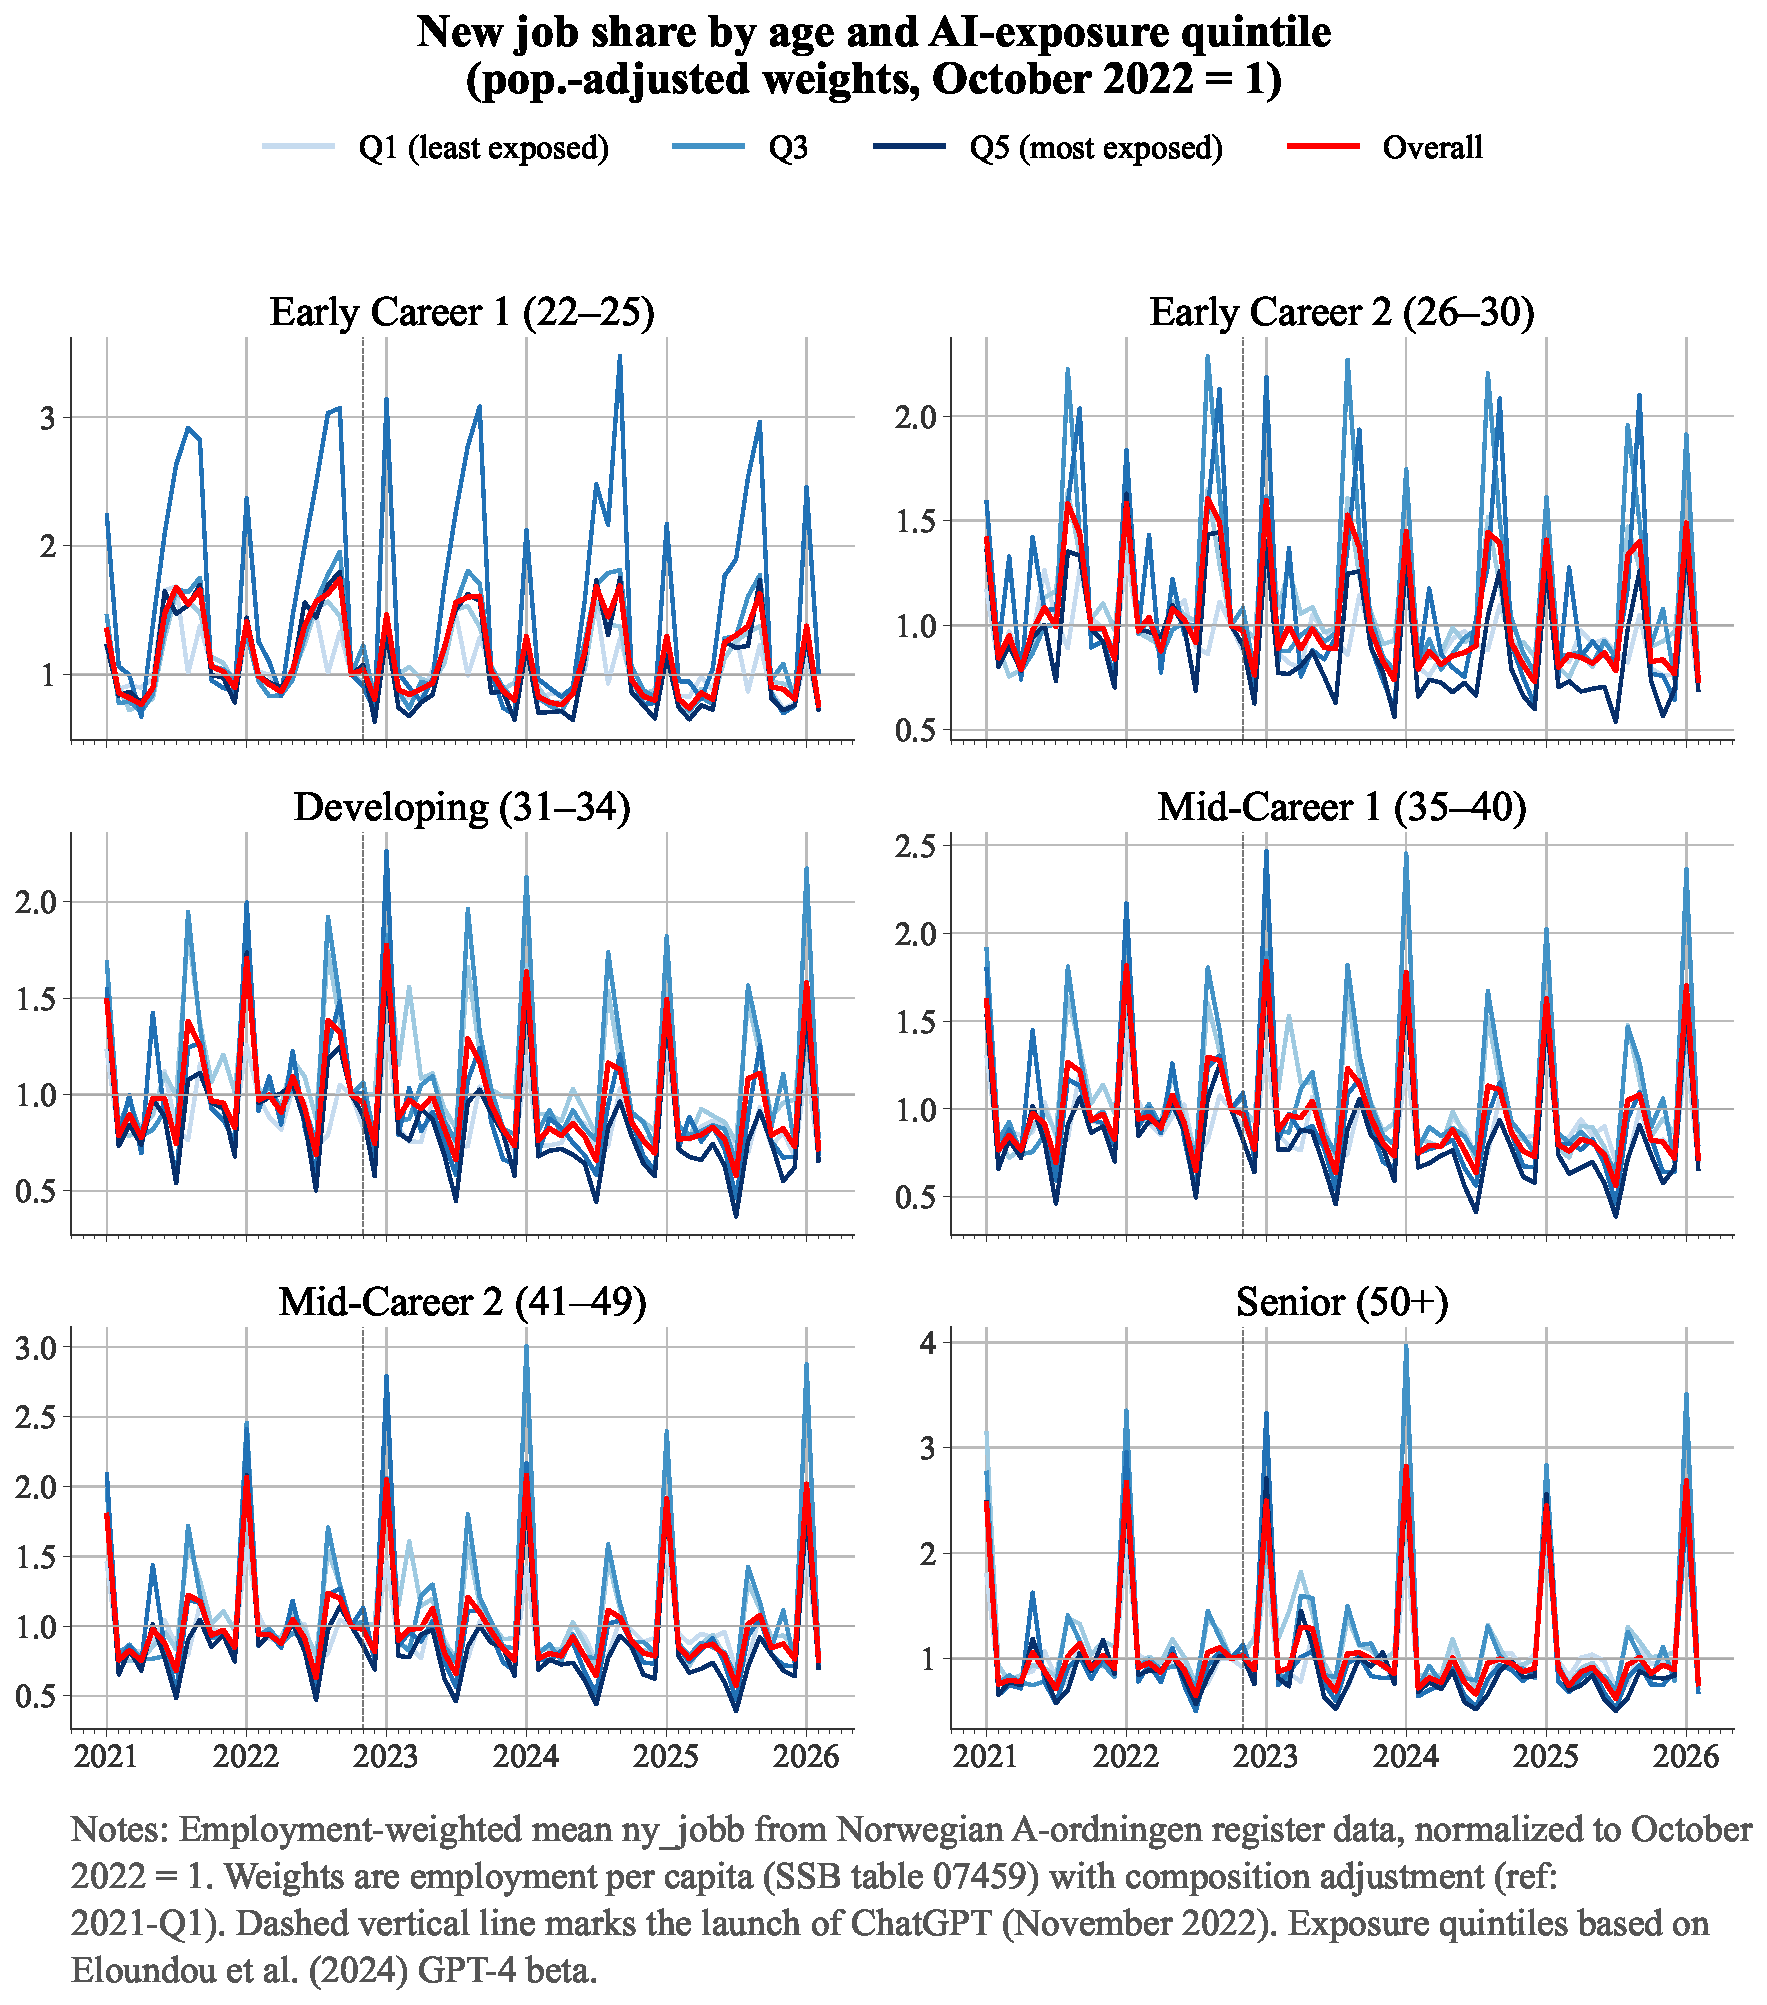
\includegraphics[width=\textwidth]{../analysis/output/figures/figure7e_ny_jobb_by_quintile.pdf}
  \caption{New job share by Eloundou et al.\ quintile and age group. October 2022 = 1.}
  \label{fig:nyjobb_by_quintile}
\end{figure}

\begin{figure}[htbp]
  \centering
  
\includegraphics[width=\textwidth]{../analysis/output/figures/figure10a_state_by_age.pdf}
  \caption{Employment by age group in selected occupations, state sector. October 2022 = 1.}
  \label{fig:state_by_age}
\end{figure}

\begin{figure}[htbp]
  \centering
  
\includegraphics[width=\textwidth]{../analysis/output/figures/figure10b_municipal_by_age.pdf}
  \caption{Employment by age group in selected occupations, municipal sector. October 2022 = 1.}
  \label{fig:municipal_by_age}
\end{figure}

\begin{figure}[htbp]
  \centering
  
\includegraphics[width=\textwidth]{../analysis/output/figures/figure10c_private_by_age.pdf}
  \caption{Employment by age group in selected occupations, private sector. October 2022 = 1.}
  \label{fig:private_by_age}
\end{figure}

\begin{figure}[htbp]
  \centering
  
\includegraphics[width=\textwidth]{../analysis/output/figures/figure11c_private_by_quintile.pdf}
  \caption{Employment by age and Eloundou et al.\ quintile, private sector. October 2022 = 1. The age-exposure gradient for 22--25 year-olds is visible in this sector.}
  \label{fig:sector_private_age}
\end{figure}

\begin{figure}[htbp]
  \centering
  
\includegraphics[width=\textwidth]{../analysis/output/figures/figure11b_municipal_by_quintile.pdf}
  \caption{Employment by age and Eloundou et al.\ quintile, municipal sector. October 2022 = 1. No systematic quintile gradient in any age group.}
  \label{fig:sector_municipal_age}
\end{figure}

\begin{figure}[htbp]
  \centering
  
\includegraphics[width=\textwidth]{../analysis/output/figures/figure11a_state_by_quintile.pdf}
  \caption{Employment by age and Eloundou et al.\ quintile, state sector. October 2022 = 1. No systematic quintile gradient in any age group.}
  \label{fig:sector_state_age}
\end{figure}

\phantomsection
\addcontentsline{toc}{section}{Appendix B: Job Dimensionality Split}
\section*{Appendix B: Job Dimensionality Split}\label{app:dimensionality}

Figure~\ref{fig:dimensionality} addresses the O-ring / job-dimensionality prediction of \citet{gans2025} and \citet{imas2026}: when tasks are quality complements rather than independent, average exposure is a poor summary of adjustment, and any movement should concentrate in occupations with high exposure and a small task set, where automation of a few tasks covers most of the job. We split occupations at the median on Eloundou et al.\ exposure and on the number of O*NET task statements (median of 22 tasks), and plot normalized employment for workers aged 22--25 in each of the four quadrants. Residual SOC codes ending in ``99'' have artificially inflated task counts and are excluded from the task-count split.

Both high-exposure quadrants decline relative to the low-exposure quadrants, and the difference between high-exposure/few-tasks ($-3.5\%$) and high-exposure/many-tasks ($-3.9\%$) is small (October 2022 to December 2025). The dominant margin is exposure level, not task count. Low-exposure occupations with few tasks grow ($+2.9\%$).

The dimensionality split therefore provides limited descriptive support for the O-ring prediction in the current early-adoption window. We note the measurement caveats: a raw count of O*NET task statements does not capture the complementarity structure central to the O-ring model, the count may reflect coding granularity rather than true job complexity, and the median split is coarse. Alternative operationalizations (task-importance weighting, task similarity, or using the Handa et al.\ automation share as a proxy for substitutability) might deliver a different picture.

\begin{figure}[htbp]
  \centering
  
\includegraphics[width=\textwidth]{../analysis/output/figures/figure12_dimensionality_2x2.pdf}
  \caption{Employment by AI exposure and job dimensionality, workers aged 22--25. Occupations are split at the median on Eloundou et al.\ exposure and on O*NET task count (22 tasks).}
  \label{fig:dimensionality}
\end{figure}
